\chapter{Introduction}
\begin{description}
	\item[Instrumentation] technique visant à créer un système d'acquisition de données ou de commande à base de capteurs, conditionneurs, régulateurs et actionneurs.
\end{description}
\section{Chaîne d’acquisition}
Une chaîne d'acquisition est «~un système électronique permettant d'exploiter une grandeur physique~»\footnote{\url{https://fr.wikipedia.org/wiki/Cha\%C3\%AEne_d\%27acquisition}}
\subsection{Composition}
\begin{figure}[H] 
	\centering 
	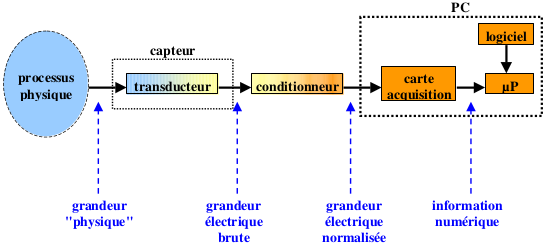
\includegraphics[width=.8\textwidth]{ch1/image1}
	\caption{Vue «~fonctionnelle~» (cas standard)} 
\end{figure}
\subsection{Transducteur et capteur}
\begin{description}
	\item[Transducteur] dispositif qui réalise intrinsèquement la conversion de la grandeur à mesurer en une grandeur électrique "brute" (plus facile à exploiter).
	\item[Capteur] protection mécanique du transducteur (+ parfois une partie du conditionnement).
\end{description}
Un transducteur utilise des phénomènes multi-physiques comme la thermoélectricité et la magnétorésistance. Il sera donc constitué la plupart du temps d'un matériau particulier\\
\danger\ Abus de langage entre transducteur et capteur \danger
\subsection{Conditionneur}
\begin{description}
	\item[Conditionneur] dispositif assurant la conversion de la grandeur électrique de sortie du transducteur (brute) en une grandeur électrique exploitable par l'organe de traitement.
\end{description}
Ce sera donc un montage électronique. Il pourra néanmoins assurer d'autres fonctions comme l'amplification ou le multiplexage.
\subsubsection{Multiplexage}
Il arrivera souvent de n'avoir qu'un seul organe de traitement pour plusieurs capteurs. Il faudra donc multiplexer\footnote{«~Assembler des signaux indépendants en un seul signal composite à partir duquel ils peuvent être restitués.~» (\url{https://fr.wiktionary.org/wiki/multiplexer})} les signaux dans le temps.\\
La fonction de multiplexage peut être assurée par le conditionneur, la carte d'acquisition ou un organe spécifique
\begin{figure}[H] 
	\centering 
	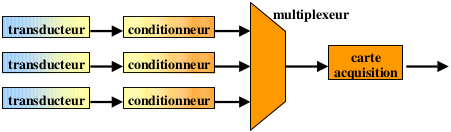
\includegraphics[width=.7\textwidth]{ch1/image2}
	\caption{Multiplexage}
\end{figure}
\subsection{Organe de traitement}
L'organe de traitement est dans le langage courant un appareil de mesure ou un assemblage type «~ordinateur + carte d'acquisition + logiciel~» dont les principales fonctions sont:
\begin{itemize}
	\item la lecture par l'utilisateur de la grandeur à mesurer
	\item le traitement du signal
	\item l'utilisation dans une régulation/commande
	d'actionneurs
\end{itemize}
\subsubsection{Carte d'acquisition}
Une carte d'acquisition est un périphérique informatique assurant l'acquisition, par un PC, de la grandeur de sortie du conditionneur dont les principales fonctions sont:
\begin{itemize}
	\item la communication avec le processeur (driver)
	\item la conversion analogique/numérique (résolution et fréquence d’échantillonnage)
	\item d'autres fonctions comme le multiplexage et les I/O numériques
\end{itemize}
\section{Rappels d'électricité et d'électronique}
Tout ceci n'est qu'un n\up{ème} rappel, je vous invite donc à lire cette partie du paquet de slides n$^\circ$1 (Introduction) à partir de la p.22 (slide 49) si vous n'êtes pas à l'aise avec ces principes (adaptation d'impédance, équivalent de Thévenin, AOP, semi-conducteurs).